\chapter{Reverse engineering of simple \IT{fortune} program indexing file}

(This part was first appeared in my blog at 25-Apr-2015.)

\IT{fortune} is well-known UNIX program which shows random phrase from a collection.
Some geeks are often set up their system in such way, so \IT{fortune} can be called after logging on.
\IT{fortune} takes phrases from the text files laying in \IT{/usr/share/games/fortunes} (as of Ubuntu Linux).
Here is example (\q{fortunes} text file):

\begin{lstlisting}
A day for firm decisions!!!!!  Or is it?
%
A few hours grace before the madness begins again.
%
A gift of a flower will soon be made to you.
%
A long-forgotten loved one will appear soon.

Buy the negatives at any price.
%
A tall, dark stranger will have more fun than you.
%
...
\end{lstlisting}

So it is just phrases, sometimes multiline ones, divided by percent sign.
The task of \IT{fortune} program is to find random phrase and to print it.
In order to achieve this, it should scan the whole text file, count phrases, choose random and print it.
But the text file can get bigger, and even on modern computers, this naive algorithm is a bit uneconomical to computer resources.
The straightforward way is to keep binary index file containing offset of each phrase in text file.
With index file, \IT{fortune} program can work much faster: just to choose random index element, take offset from there, set offset in text file and read phrase from it.
This is actually done in \IT{fortune} file.
Let's inspect what is in its index file inside (these are .dat files in the same directory) in hexdecimal editor.
This program is open-source of course, but intentionally, I will not peek into its source code.

\lstinputlisting{ff/fortune/1.lst}

Without any special aid we could see that there are four 4-byte elements on each 16-byte line.
It's probably our index array.
I'm trying to load the whole file in Wolfram Mathematica as 32-bit integer array:

\begin{lstlisting}
In[]:= BinaryReadList["c:/tmp1/fortunes.dat", "UnsignedInteger32"]

Out[]= {33554432, 2936078336, 3137339392, 251658240, 0, 37, 0, \
721420288, 1610612736, 2399141888, 3741319168, 335609856, 1208025088, \
2080440320, 2868969472, 3858825216, 537001984, 989986816, 2046951424, \
3305242624, 67305472, 1023606784, 1745027072, 2801991680, 3775070208, \
419692544, 755236864, 2130968576, 2902720512, 3573809152, 84213760, \
990183424, 1678049280, 2181365760, 2902786048, 3456434176, \
4144300032, 470155264, 1627783168, 2047213568, 3506831360, 168230912, \
1392967680, 2584150016, 4161208320, 654835712, 1493696512, \
2332557312, 2684878848, 3288858624, 3775397888, 4178051072, \
...
\end{lstlisting}

Nope, something wrong. Numbers are suspiciously big.
But let's back to \IT{od} output: each common 4-byte element has two zero bytes and two non-zero bytes, so the offsets (at least at the beginning of the file) are 16-bit at maximum.
Probably different endiannes is used in file?
Default endiannes in Mathematica is little-endian, as used in Intel CPUs.
Now I'm changing it to big-endian:

\begin{lstlisting}
In[]:= BinaryReadList["c:/tmp1/fortunes.dat", "UnsignedInteger32", 
 ByteOrdering -> 1]

Out[]= {2, 431, 187, 15, 0, 620756992, 0, 43, 96, 143, 223, 276, \
328, 380, 427, 486, 544, 571, 634, 709, 772, 829, 872, 935, 993, \
1049, 1069, 1151, 1197, 1237, 1285, 1339, 1380, 1410, 1453, 1486, \
1527, 1564, 1633, 1658, 1745, 1802, 1875, 1946, 2040, 2087, 2137, \
2187, 2208, 2244, 2273, 2297, 2343, 2371, 2425, 2467, 2531, 2581, \
2637, 2654, 2698, 2726, 2751, 2799, 2840, 2883, 2913, 2958, 3023, \
3066, 3131, 3174, 3205, 3257, 3282, 3330, 3387, 3431, 3500, 3552, \
...
\end{lstlisting}

Yes, this is something readable.
I choose random element (3066) which is 0xBFA in hexadecimal form.
I'm opening 'fortunes' text file in hex editor, I'm setting 0xBFA as offset and I see this phrase:

\lstinputlisting{ff/fortune/2.lst}

Or:

\begin{lstlisting}
Do what comes naturally.  Seethe and fume and throw a tantrum.
%
\end{lstlisting}

Other offset are also can be checked, yes, they are valid offsets.

I can also check in Mathematica that each subsequent element is bigger than previous.
I.e., the array is ascending.
In mathematics lingo, this is called \IT{strictly increasing monotonic function}.

\begin{lstlisting}
In[]:= Differences[input]

Out[]= {429, -244, -172, -15, 620756992, -620756992, 43, 53, 47, \
80, 53, 52, 52, 47, 59, 58, 27, 63, 75, 63, 57, 43, 63, 58, 56, 20, \
82, 46, 40, 48, 54, 41, 30, 43, 33, 41, 37, 69, 25, 87, 57, 73, 71, \
94, 47, 50, 50, 21, 36, 29, 24, 46, 28, 54, 42, 64, 50, 56, 17, 44, \
28, 25, 48, 41, 43, 30, 45, 65, 43, 65, 43, 31, 52, 25, 48, 57, 44, \
69, 52, 62, 73, 62, 53, 37, 68, 71, 50, 41, 57, 69, 58, 70, 45, 54, \
38, 45, 50, 42, 61, 47, 43, 62, 189, 61, 56, 30, 85, 63, 48, 61, 58, \
81, 50, 55, 63, 83, 80, 49, 42, 94, 54, 67, 81, 52, 57, 68, 43, 28, \
120, 64, 53, 81, 33, 82, 88, 29, 61, 32, 75, 63, 70, 47, 101, 60, 79, \
33, 48, 65, 35, 59, 47, 55, 22, 43, 35, 102, 53, 80, 65, 45, 31, 29, \
69, 32, 25, 38, 34, 35, 49, 59, 39, 41, 18, 43, 41, 83, 37, 31, 34, \
59, 72, 72, 81, 77, 53, 53, 50, 51, 45, 53, 39, 70, 54, 103, 33, 70, \
51, 95, 67, 54, 55, 65, 61, 54, 54, 53, 45, 100, 63, 48, 65, 71, 23, \
28, 43, 51, 61, 101, 65, 39, 78, 66, 43, 36, 56, 40, 67, 92, 65, 61, \
31, 45, 52, 94, 82, 82, 91, 46, 76, 55, 19, 58, 68, 41, 75, 30, 67, \
92, 54, 52, 108, 60, 56, 76, 41, 79, 54, 65, 74, 112, 76, 47, 53, 61, \
66, 53, 28, 41, 81, 75, 69, 89, 63, 60, 18, 18, 50, 79, 92, 37, 63, \
88, 52, 81, 60, 80, 26, 46, 80, 64, 78, 70, 75, 46, 91, 22, 63, 46, \
34, 81, 75, 59, 62, 66, 74, 76, 111, 55, 73, 40, 61, 55, 38, 56, 47, \
78, 81, 62, 37, 41, 60, 68, 40, 33, 54, 34, 41, 36, 49, 44, 68, 51, \
50, 52, 36, 53, 66, 46, 41, 45, 51, 44, 44, 33, 72, 40, 71, 57, 55, \
39, 66, 40, 56, 68, 43, 88, 78, 30, 54, 64, 36, 55, 35, 88, 45, 56, \
76, 61, 66, 29, 76, 53, 96, 36, 46, 54, 28, 51, 82, 53, 60, 77, 21, \
84, 53, 43, 104, 85, 50, 47, 39, 66, 78, 81, 94, 70, 49, 67, 61, 37, \
51, 91, 99, 58, 51, 49, 46, 68, 72, 40, 56, 63, 65, 41, 62, 47, 41, \
43, 30, 43, 67, 78, 80, 101, 61, 73, 70, 41, 82, 69, 45, 65, 38, 41, \
57, 82, 66}
\end{lstlisting}

As we can see, except of the very first 6 values (which is probably belongs to index file header), all numbers are in fact length of all text phrases (offset of the next phrase minus offset of the current phrase is in fact length of the current phrase).

It's very important to keep in mind that bit-endiannes can be confused with incorrect array start.
Indeed, from \IT{od} output we see that each element started with two zeroes.
But when shifted by two bytes in either side, we can interpret this array as little-endian:

\lstinputlisting{ff/fortune/3.lst}

If we would interpret this array as little-endian, the first element is 0x4801, second is 0x7C01, etc.
High 8-bit part of each of these 16-bit values are seems random to us, and the lowest 8-bit part is seems ascending.

But I'm sure that this is big-endian array, because the very last 32-bit element of the file is big-endian 
(\IT{00 00 5f c4} here):

\lstinputlisting{ff/fortune/4.lst}

Perhaps, \IT{fortune} program developer had big-endian computer or maybe it was ported from something like it.

OK, so the array is big-endian, and, judging by common sense, the very first phrase in the text file should be started at zeroth offset. So zero value should be present in the array somewhere at the very beginning.
We've got couple of zero elements at the beginning. But the second is most appealing: 43 is going right after it and 43 is valid offset to valid English phrase in the text file.

The last array element is 0x5FC4, and there are no such byte at this offset in the text file.
So the last array element is pointing behind the end of file.
It's probably done because phrase length is calculated as difference between offset to the current phrase
and offset to the next phrase. 
This can be faster than traversing phrase string for percent character.
But this wouldn't work for the last element.
So the \IT{dummy} element is also added at the end of array.

So the first 6 32-bit integer values are probably some kind of header.

Oh, I forgot to count phrases in text file:

\lstinputlisting{ff/fortune/5.lst}

The number of phrases can be present in index, but may be not.
In case of very simple index files, number of elements can be easily deduced from index file size.
Anyway, there are 432 phrases in the text file.
And we see something very familiar at the second element (value 431).
I've checked other files (literature.dat and riddles.dat in Ubuntu Linux) and yes, the second 32-bit element is indeed number of phrases minus 1.
Why \IT{minus 1}? Probably, this is not number of phrases, but rather index of the last phrase (starting at zero)?

And there are some other elements in the header.
In Mathematica, I'm loading each of three available files and I'm taking a look on the header:

\begin{figure}[H]
\centering
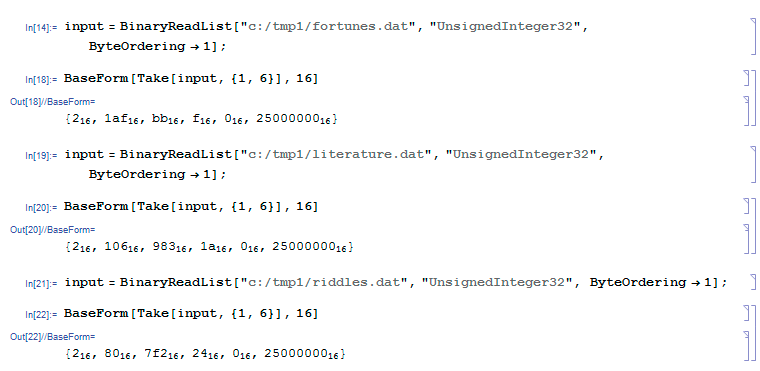
\includegraphics[scale=\FigScale]{ff/fortune/mathematica.png}
\end{figure}

I have no idea what other values mean, except the size of index file.
Some fields are the same for all files, some are not.
From my own experience, there could be:

\begin{itemize}
\item file signature;
\item file version;
\item checksum;
\item some other flags;
\item maybe even text language identifier;
\item text file timestamp, so \IT{fortune} program will regenerate index file if user added some new phrase(s) to it.
\end{itemize}

For example, Oracle .SYM files (\myref{Oracle_SYM_files_example}) which contain symbols table for DLL files, also contain timestamp of corresponding DLL file, so to be sure it is still valid.
But there are still possibility that the index file is regenerated if modification time of index file is older than text file.
On the other hand, text file and index file timestamps can gone out of sync after archiving/unarchiving/installing/deploying/etc.

But there are no timestamp, in my opinion. The most compact way of representing date and time is UNIX time value, which is big 32-bit number. We don't see any of such here. Other ways are even less compact.

So here is algorithm, how \IT{fortune} probably works:

\begin{itemize}
\item take number of last phrase from the second element;
\item generate random number in range of 0..number\_of\_last\_phrase;
\item find corresponding element in array of offsets, take also following offset;
\item output to \IT{stdout} all characters from the text file starting at current offset until
the next offset minus 2 (so to ignore terminating percent sign 
and character of the following phrase).
\end{itemize}

\section{Hacking!}

Let's try to check some of our assumtpions.
I will create this text file under the path and name \IT{/usr/share/games/fortunes/fortunes}:

\begin{lstlisting}
Phrase one.
%
Phrase two.
%
\end{lstlisting}

Then this forunes.dat file. I take header from the original fortunes.dat, I changed second field (count of all phrases) to zero and I left two
elements in the array: 0 and 0x1c, because the whole length of the text \IT{fortunes} file is 28 (0x1c) bytes:

\lstinputlisting{ff/fortune/6.lst}

Now I run it:

\lstinputlisting{ff/fortune/7.lst}

Something wrong. Let's change the second field to 1:

\lstinputlisting{ff/fortune/8.lst}

Now it works. It's always shows only the first phrase:

\lstinputlisting{ff/fortune/9.lst}

Hmmm. Let's leave only one element in array (0) without terminating one:

\lstinputlisting{ff/fortune/10.lst}

Fortune program always shows only first phrase.

From this experiment we got to know that percent sign is parsed inside of fortune file and the size is not calculated as I deduced,
perhaps, even terminal array element is not used.
However, it's still possible use it. And probably it was in past?

% TODO second phrase!

\section{The files}

For the sake of demonstration, I still didn't take a look in \IT{fortune} source code.
If you want to try to understand meaning of other values in index file header, you may try to achieve it without looking into source code as well.
Files I took from Ubuntu Linux 14.04 are here: \url{http://beginners.re/examples/fortune/}, hacked files are also here.

Oh, and I took the files from x64 version of Ubuntu, but array elements are still has size of 32 bit.
It is because \IT{fortune} text files are probably never exceeds 4GB size.
But if it will, all elements must have size of 64 bit so to be able to store offset to the text file larger than 4GB.

For impatient readers, the source code of \IT{fortune} is \href{https://launchpad.net/ubuntu/+source/fortune-mod/1:1.99.1-3.1ubuntu4}{here}.

